\documentclass[Thesis.tex]{subfiles}
\begin{document}
\chapter{Liquid $^4$He}
\label{chp:liquid-helium}

We turn now to the much more challenging system of liquid Helium, presented
in~\cref{sec:liquid-helium-theory}. As before, we will first present the
benchmark result followed by the neural networks.


\section{Benchmark}

We will use one of the simpler benchmark wave functions for this system, known
as the McMillan form wave function~\cite{McMillan-1965}:

\begin{align}
  \label{eq:McMillan-wave-function-def}
  \psi_{M} &= \exp(-\frac{1}{2}\sum_{i<j} \qty(\frac{\beta}{r_{ij}})^5).
\end{align}
where $\beta$ is the only variational parameter and has units of angstrom. An
important observation now is the lack of any single particle wave function
factor. In the case of the Quantum Dot we had a Gaussian localized at the origin
as a result of the potential well. This system, however, is infinite and
periodic without any such influence driving it towards particular points in
space. Furthermore, because of the lack of an external field the single particle
solutions are just free particles, and does not help us understand the many-body
system.

\subsection{Finite Size Dependency}

An important aspect of all the results that we will present is that they are
highly dependent on the number of particles used in the simulation box, as well
as the size of the box it self. We will hold the number density of particles
constant, $\rho = \flatfrac{\num{0.365}}{\sigma^3}$ (where $\sigma =
\SI{2.556}{\angstrom}$ as defined in \cref{eq:Lennard-Jones-def}), and set the
side lengths of the simulation box, $L$, depending on
the number of particles $N$:

\begin{align}
  L = \sqrt[3]{\frac{N}{\rho}}.
\end{align}

\noindent As the assumption of periodicity is a simplifying approximation, we
introduce some erroneous effects because of it. These generally disappear as we
increase the number of particles (and hence the size of box), but the
computation time needed to run the simulations increase significantly with
increasing numbers. The purpose of the following analysis is to test the
\emph{relative} accuracy of different wave functions. With that in mind we have
used a small number of particles in the main results, which introduces a
significant error. The number of particles should still be large enough to
introduce all the relevant effects and produce valid test results.


\subsection{Optimizing}

We have optimized~\cref{eq:McMillan-wave-function-def} using $\num{10000}$
iterations of $\num{5000}$ MC cycles each. We used standard Metropolis sampling
along with the ADAM optimizer. \cref{fig:He-benchmark-training} shows the
progression of both the energy and variational parameter during training.
Because of the strong correlations involved, there is significantly more
variance in these results compared to the benchmark used for Quantum Dots. We
see the value for $\beta$ oscillating without any indication of converging to a
fixed value.

\cref{tab:He-benchmark-results} show the energy estimates from the final model.
The same wave function (i.e. same value for $\beta$) has also been used on
different number of particles to illustrate how the energy increases for larger
systems. Based on computations with larger and larger systems, the value for $N
= 256$ is quite close to the apparent convergence for $N\to\infty$.

\begin{figure}[h]
  \centering
  \resizebox{\linewidth}{!}{%
    % This file was created by matplotlib2tikz v0.7.4.
\begin{tikzpicture}

\definecolor{color0}{rgb}{0.12156862745098,0.466666666666667,0.705882352941177}

\begin{groupplot}[group style={group size=2 by 1}]
\nextgroupplot[
tick align=outside,
tick pos=left,
x grid style={white!69.01960784313725!black},
xlabel={\% of training},
xmin=-5, xmax=105,
xtick style={color=black},
ylabel={Ground state energy $[\si{\kelvin\per N}]$},
y grid style={white!69.01960784313725!black},
ymin=-6.85219168043208, ymax=-5.76372161210776,
ytick style={color=black},
ylabel near ticks,
]
\addplot [semithick, color0]
table {%
0 -5.81319752430432
1 -5.93452622568609
2 -6.00858962108258
3 -6.08665800506619
4 -6.20773427507232
5 -6.23156670870654
6 -6.25285373896968
7 -6.36683025632103
8 -6.36485217914965
9 -6.42748677702066
10 -6.50039764982493
11 -6.52719360265819
12 -6.56717088511529
13 -6.55506196487281
14 -6.60944841435202
15 -6.58072330140416
16 -6.60677852644892
17 -6.61647256171949
18 -6.70160055491517
19 -6.69863368699099
20 -6.69635189000038
21 -6.72593561696231
22 -6.68343964270742
23 -6.7429087393482
24 -6.71851493402437
25 -6.7345213413159
26 -6.71034228662546
27 -6.74732848543959
28 -6.72175233470759
29 -6.75688969206912
30 -6.74660417455725
31 -6.72846362943138
32 -6.7587149797462
33 -6.75693148879914
34 -6.76258422232693
35 -6.75085981956242
36 -6.74387871373416
37 -6.74109156636538
38 -6.77243478754695
39 -6.74052798320351
40 -6.74424094866635
41 -6.76775739672773
42 -6.7559919917146
43 -6.75039426906645
44 -6.75370511228573
45 -6.75896538263834
46 -6.74032690549759
47 -6.78997769653142
48 -6.73115803993219
49 -6.75099235927379
50 -6.76689812871345
51 -6.74849882697142
52 -6.7674145141362
53 -6.78131648574984
54 -6.75906095822701
55 -6.77784471235837
56 -6.79117471226126
57 -6.80271576823552
58 -6.77509213456717
59 -6.78716474735426
60 -6.74039641661558
61 -6.79239158305779
62 -6.75498454590202
63 -6.7634873982812
64 -6.73744637804431
65 -6.75774478925854
66 -6.77807578595877
67 -6.76413401844244
68 -6.73777049704596
69 -6.76212594901964
70 -6.75869381525464
71 -6.75888649214504
72 -6.74197262277744
73 -6.76612166760104
74 -6.75684274744045
75 -6.7378847148746
76 -6.74540734816332
77 -6.71361620588114
78 -6.75982157137573
79 -6.75084877076814
80 -6.762793676612
81 -6.74920050658278
82 -6.74846814015804
83 -6.77019406086908
84 -6.7484431760123
85 -6.76377512756983
86 -6.77395128912729
87 -6.77676908332129
88 -6.73673374230908
89 -6.76674164837398
90 -6.78038626616403
91 -6.77584777447017
92 -6.71076974724152
93 -6.76035815397443
94 -6.76350918211843
95 -6.76389862072772
96 -6.77110719678763
97 -6.75714843483792
98 -6.77043867917657
99 -6.71547668584384
100 -6.75350211816952
};

\nextgroupplot[
legend cell align={left},
legend style={at={(0.03,0.97)}, anchor=north west, draw=white!80.0!black},
tick align=outside,
tick pos=left,
x grid style={white!69.01960784313725!black},
xlabel={\% of training},
xmin=-5, xmax=105,
xtick style={color=black},
y grid style={white!69.01960784313725!black},
ymin=2.84311677655944, ymax=2.99454769225178,
ytick style={color=black},
ylabel={Variational parameter $\beta$ $[\si{\angstrom}]$},
ylabel style={rotate=-180},
ylabel near ticks,
ytick pos=right,
ylabel style={rotate=-180},
]
\addplot [semithick, color0]
table {%
0 2.85
1 2.85771877343818
2 2.8650426908874
3 2.87229961410334
4 2.87926515215211
5 2.88600281382441
6 2.89220140344377
7 2.89851875286748
8 2.90461755434636
9 2.91032476320017
10 2.91576989197661
11 2.92094435853081
12 2.9257935546088
13 2.93056536447931
14 2.93519788266342
15 2.93954634850754
16 2.94358583039877
17 2.94736833558584
18 2.95086530798089
19 2.95416009410758
20 2.95708246669139
21 2.96029424262311
22 2.96278729802401
23 2.96542975622013
24 2.96776088038637
25 2.96983502291505
26 2.97132900145053
27 2.97319498626816
28 2.97425428304438
29 2.97573496432073
30 2.97692893065558
31 2.97799918989409
32 2.9790535423368
33 2.98027251536911
34 2.98139610222615
35 2.98216419975245
36 2.98245071983135
37 2.98261528393402
38 2.98317005753593
39 2.98285828689244
40 2.98328409623724
41 2.98327184277541
42 2.98420872487105
43 2.98431102032459
44 2.98405545942704
45 2.98402716102763
46 2.98451107624493
47 2.98442284296482
48 2.98439045174919
49 2.98511270289013
50 2.98579429264609
51 2.98567717994044
52 2.98552782748783
53 2.98537803518609
54 2.98563125652273
55 2.98528049661546
56 2.98571231758376
57 2.98452772127367
58 2.98503960591317
59 2.98510299685132
60 2.98422617030646
61 2.98458841600336
62 2.98438973868782
63 2.98391334292601
64 2.98392097606065
65 2.98348805264952
66 2.98369115789756
67 2.98414733320096
68 2.98384692930286
69 2.98464229582106
70 2.98463036262134
71 2.98373567379686
72 2.98371158378309
73 2.98488136139775
74 2.9846521395285
75 2.9844328413153
76 2.98505392018769
77 2.98615577858719
78 2.98685090647166
79 2.98766446881122
80 2.98694631552791
81 2.98518517959941
82 2.98491799512055
83 2.98543572667322
84 2.98534325008699
85 2.98519634670357
86 2.98435857464363
87 2.98409743281243
88 2.9841897962539
89 2.98410842090462
90 2.98508744369597
91 2.98502255078322
92 2.98467748255916
93 2.98470976363276
94 2.98553663644782
95 2.98647577600856
96 2.98416967633852
97 2.98447136823118
98 2.98537649056117
99 2.98571613177779
100 2.9855315339833
};
\end{groupplot}

\end{tikzpicture}
  }
  \caption[Learning progression of McMillan wave function on $^4$He]{\label{fig:He-benchmark-training}Left: Ground state energy produced by~\cref{eq:McMillan-wave-function-def}
    as a function of training steps. Right: Progression of the variational
    parameter $\beta$ of~\cref{eq:McMillan-wave-function-def} as a function of
    training steps. A convergence is clearly visible, although there is more
    variance in the value for $\beta$ compared to the parameters of the
    benchmark used for Quantum Dots.\citesource{writing/scripts/He-benchmark.py}}
\end{figure}

\begin{table}[h]
  \centering
  \caption[Energy estimates of McMillan wave function on $^4$He]{\label{tab:He-benchmark-results}Predicted ground state energy of helium atoms at density $\rho =
\flatfrac{0.365}{\sigma^3}$ using $\psi_{M}$ with $\beta$ as determined after training. The number of particles used in the simulation box
is indicated by the superscript on $\psi_M$. Values obtained using $2^{22}$
Monte Carlo samples. See \cref{fig:He-benchmark-training} for source code reference.}
  \begin{tabular}{lS[table-format=1.5]*2{S[table-format=1.3]}*2{S[table-format=1.1]}}
\toprule
\addlinespace
& {$\langle E_L\rangle$} & {CI$^{95}_-$} & {CI$^{95}_+$} & {Std} & {Var} \\
\addlinespace
\midrule
\addlinespace
\addlinespace
    $\psi_M^{(32)}$ & -6.76(1) & -6.79 & -6.74 & \num{4.6e-01} & \num{2.1e-01}\\
$\psi_M^{(64)}$ & -6.15(1) & -6.18 & -6.12 & \num{3.0e-01} & \num{9.1e-02}\\
$\psi_M^{(256)}$ & -5.848(10) & -5.867 & -5.829 & \num{2.2e-01} & \num{4.7e-02}\\
\addlinespace\addlinespace\bottomrule
\end{tabular}
\end{table}
\clearpage


\section{Neural Networks}

We again attempt to apply a neural network to our wave function representation.
Liquid $^4$He is a far more challenging problem compared to the two-particle
quantum dot, and as such it will serve as an important test of the capabilities
of neural networks for general quantum mechanical many-body problems.

As before, we have not simply removed the original wave function, but rather
added the network as another correlation factor:

\begin{align}
  \label{eq:helium-dnn-mcmillan-def}
  \psi_{DNN}(\mat X) &= \psi_M(\mat X)\,f(\mat X),
\end{align}
where once again $f: \mathbb{R}^{N\times D}\to\mathbb{R}$ represents an
arbitrary neural network.

Lastly, we limit our investigation to $N=32$ particles and still with density
$\rho=\flatfrac{0.365}{\sigma^3}$. This is done from a practical standpoint,
considering the substantial computational cost.

\subsection{Network Architecture}

The proposed network structure is one of many that are likely to perform well,
and in all likelihood this is not the optimal form. A more in depth analysis of
what structures perform best, including other types of networks (e.g.\ recurrent,
convolutional, residual etc.) is left for future research.\\

Based on the experimental results observed for quantum dots, in conjunction with
trail and error, we have used the following network structure:

\begin{center}
  \begin{tabular}{lcc}
    \toprule
    \addlinespace
    Layer & Nodes & Activation\\
    \addlinespace
    \midrule
    \addlinespace
    \addlinespace
    Input & 96 & ---\\
    Hidden 1& 144 & $\tanh$\\
    Hidden 2& 36 & $\tanh$\\
    Output & 1 & $\exp$\\
    \addlinespace
    \addlinespace
    \bottomrule
  \end{tabular}
\end{center}
Once again the number of nodes in the input layer is fixed by the number of
degrees of freedom ($D\times N$ for $D$ dimensions). The number of nodes in the
second layer is somewhat arbitrary, and could be changed. Importantly it is
larger than $96$, allowing the network to learn more features. Still, it is not
enough nodes to fully encode the relative difference between every pair of
coordinates, as would be required to reproduce $\psi_M$ fully. This number was
found to be large enough to allow learning, but still be reasonably efficient.
Lastly, the second hidden layer was set to $36$ nodes. This is also somewhat
arbitrary, but importantly it is smaller than $144$, allowing the gradual
narrowing down to the single output. The activation functions are the same as
those used for quantum dots.

Finally, based on the success of applying sorting on the inputs to the network
to impose symmetry we will reuse this strategy here. The wave function with
input sorting applied is denoted as $\psi_{SDNN}$.

\subsection{Optimization}

We produced the following results by optimizing $\psi_M$ and $\psi_{SDNN}$ with
similar hyperparameters. We initialized $\beta=\num{2.85}$ for both wave functions
for a fair comparison. We used $\num{250000}$ training iterations of
$\num{5000}$ MC cycles each. Contrary to the quantum dot system, where a large
set of hyperparameters yielded good results, we have found this problem to be
highly sensitive to good hyperparameters. We had to reduce the learning rate to
$\eta=\num{0.0001}$ to avoid divergence during training. We also found that the
networks performed better with a small degree of L2 regularization,
$\gamma=\num{0.00001}$. While other choices might still be better, there were
significantly less room for error in this much more challenging problem.

\begin{figure}[h]
  \centering
  % This file was created by matplotlib2tikz v0.7.4.
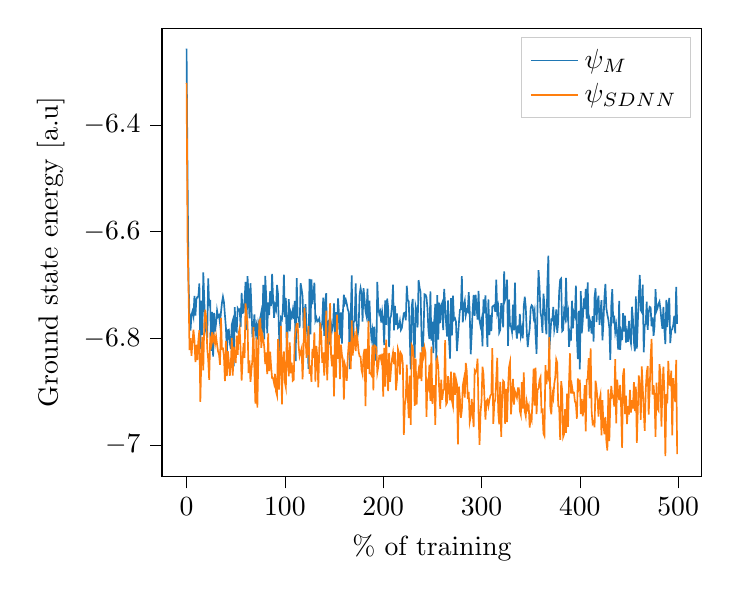
\begin{tikzpicture}

\definecolor{color0}{rgb}{0.12156862745098,0.466666666666667,0.705882352941177}
\definecolor{color1}{rgb}{1,0.498039215686275,0.0549019607843137}
\definecolor{color2}{rgb}{0.172549019607843,0.627450980392157,0.172549019607843}
\definecolor{color3}{rgb}{0.83921568627451,0.152941176470588,0.156862745098039}
\definecolor{color4}{rgb}{0.580392156862745,0.403921568627451,0.741176470588235}
\definecolor{color5}{rgb}{0.549019607843137,0.337254901960784,0.294117647058824}
\definecolor{color6}{rgb}{0.890196078431372,0.466666666666667,0.76078431372549}
\definecolor{color7}{rgb}{0.737254901960784,0.741176470588235,0.133333333333333}
\definecolor{color8}{rgb}{0.0901960784313725,0.745098039215686,0.811764705882353}

\begin{axis}[
legend cell align={left},
legend style={draw=white!80.0!black},
tick align=outside,
tick pos=left,
x grid style={white!69.01960784313725!black},
xlabel={\% of training},
xmin=-24.95, xmax=523.95,
xtick style={color=black},
y grid style={white!69.01960784313725!black},
ylabel={Ground state energy [a.u]},
ymin=-7.05951553745272, ymax=-6.21815498548895,
ytick style={color=black}
]
\addplot [semithick, color0]
table {%
0 -6.25639864694185
1 -6.50012049647671
2 -6.69059308265573
3 -6.76067497912833
4 -6.78575633412781
5 -6.75602483890127
6 -6.74927602374864
7 -6.75885384270427
8 -6.72058226039468
9 -6.75748781428864
10 -6.72666843895116
11 -6.72241121723166
12 -6.7216696458745
13 -6.69714066756281
14 -6.82048311604673
15 -6.72918707202692
16 -6.79423333531294
17 -6.67626036401545
18 -6.72804810626657
19 -6.78261760705013
20 -6.78830570583366
21 -6.79888762697361
22 -6.68756028096308
23 -6.73950775683174
24 -6.72794486268879
25 -6.82347999100776
26 -6.750573793527
27 -6.83428265132409
28 -6.75233262361126
29 -6.78715112785897
30 -6.77176531969879
31 -6.74798650697519
32 -6.75961770043029
33 -6.75670944762059
34 -6.77175351795562
35 -6.7513897803748
36 -6.73334457282241
37 -6.72215564955008
38 -6.73189716037668
39 -6.75660470648782
40 -6.77916539673829
41 -6.82565499438906
42 -6.78486055724577
43 -6.78395758956464
44 -6.80884632446631
45 -6.82025383010691
46 -6.77413684392182
47 -6.76702686744202
48 -6.85249750368423
49 -6.74171398437537
50 -6.78531869580338
51 -6.78755010767406
52 -6.74395552039169
53 -6.74748489785142
54 -6.74572346087898
55 -6.77908368044261
56 -6.71504721993188
57 -6.75240233787644
58 -6.75149627065513
59 -6.72768641570737
60 -6.6942652314591
61 -6.7845519329979
62 -6.68359015058654
63 -6.71718750079149
64 -6.76242426622698
65 -6.69680063091149
66 -6.74157920022681
67 -6.7982533442013
68 -6.78163106618469
69 -6.75504101913867
70 -6.78924878545171
71 -6.77769453397113
72 -6.80257216529482
73 -6.7712995590051
74 -6.77933019491927
75 -6.76113102909832
76 -6.7510970377328
77 -6.78924131191623
78 -6.69960757161877
79 -6.80185921798985
80 -6.68303688279253
81 -6.72188137548799
82 -6.79072714012954
83 -6.73254006690939
84 -6.75633225972698
85 -6.71173009763003
86 -6.73979189111982
87 -6.67938574684971
88 -6.72608370191741
89 -6.76164031042187
90 -6.73904434619432
91 -6.74594054213411
92 -6.70008754518369
93 -6.71668978904748
94 -6.79076517184438
95 -6.82353811438013
96 -6.76164336973843
97 -6.76473603780247
98 -6.74585489621847
99 -6.68076096477452
100 -6.76018876870774
101 -6.72471932638869
102 -6.8283186094116
103 -6.77650811374825
104 -6.72677561225634
105 -6.78715664751775
106 -6.75206612089997
107 -6.75866456334956
108 -6.74751985849213
109 -6.76413819486708
110 -6.72991292021512
111 -6.84283815168719
112 -6.68729628541676
113 -6.76034650353659
114 -6.76091625791746
115 -6.7801713013487
116 -6.69668346291037
117 -6.70744840666291
118 -6.72135871897071
119 -6.78137424155847
120 -6.75269618325677
121 -6.73587594789033
122 -6.77687727881406
123 -6.79505763238351
124 -6.85741950659001
125 -6.68836147448401
126 -6.79262976671399
127 -6.68948130187927
128 -6.73629264840759
129 -6.71868391221484
130 -6.69557786011305
131 -6.7665839276077
132 -6.76128053154579
133 -6.76851821294788
134 -6.76698976374622
135 -6.7631835029166
136 -6.78070845881876
137 -6.78139061369991
138 -6.77147500128054
139 -6.72376705535106
140 -6.79543353583307
141 -6.73367445181833
142 -6.71540105511661
143 -6.82546080950461
144 -6.76869097024399
145 -6.76657311867548
146 -6.8123377607252
147 -6.77289627732275
148 -6.78426988410101
149 -6.77409566116224
150 -6.73465736097027
151 -6.80446378998419
152 -6.75119321458398
153 -6.79684446145078
154 -6.72525095255782
155 -6.75350135758416
156 -6.80036173026691
157 -6.75165713514679
158 -6.81011102427171
159 -6.75185334046296
160 -6.71832033200285
161 -6.73386322283528
162 -6.72802305290155
163 -6.73573812115156
164 -6.74617895237153
165 -6.75083970925227
166 -6.85794678281942
167 -6.75892295413751
168 -6.68200093185196
169 -6.82318289399281
170 -6.7691505875528
171 -6.76714363458334
172 -6.69724086338308
173 -6.77317851797789
174 -6.79394759471305
175 -6.78033644643419
176 -6.71778311816561
177 -6.70583018736447
178 -6.71583996969006
179 -6.76864168689948
180 -6.7062004849477
181 -6.726649724706
182 -6.74921766238936
183 -6.75820823658533
184 -6.70666280996063
185 -6.76865515364949
186 -6.72920098849383
187 -6.77508133829141
188 -6.79883752239889
189 -6.78618775961947
190 -6.8176461162405
191 -6.77842087885473
192 -6.83970125062532
193 -6.84143875264027
194 -6.69410766728991
195 -6.74137408204764
196 -6.75442386663147
197 -6.74956392184209
198 -6.77065899699203
199 -6.75068175051287
200 -6.76628288793364
201 -6.81293375667406
202 -6.72901556520309
203 -6.77475645085883
204 -6.7255111697973
205 -6.74138044467272
206 -6.81661412168294
207 -6.76308044494046
208 -6.757631005788
209 -6.73889412562296
210 -6.69954394032857
211 -6.78526198675114
212 -6.73944976361794
213 -6.774686829473
214 -6.75362061362228
215 -6.78060061913137
216 -6.77884030726709
217 -6.76781150575036
218 -6.78435212429142
219 -6.78067740587477
220 -6.76558900484986
221 -6.75288751448104
222 -6.75203908382414
223 -6.76643388819645
224 -6.70151238395358
225 -6.72908729421717
226 -6.73066656086265
227 -6.79580049163414
228 -6.85815776525195
229 -6.7408297695825
230 -6.72631835880213
231 -6.79719878718085
232 -6.83674332193153
233 -6.74038977557414
234 -6.74913460810771
235 -6.77971406297484
236 -6.69080713978881
237 -6.70457136808269
238 -6.71365243297792
239 -6.79611977764098
240 -6.83106747196337
241 -6.7925343000766
242 -6.71746048821218
243 -6.71811283243591
244 -6.72291580867129
245 -6.7435106596995
246 -6.7850809309177
247 -6.80129335067589
248 -6.71197529358077
249 -6.80420479690321
250 -6.76874513406932
251 -6.82783904960245
252 -6.76465189218731
253 -6.73560867297435
254 -6.84196983525574
255 -6.7192525237169
256 -6.802584350611
257 -6.73329735463489
258 -6.77136899141424
259 -6.73874623700086
260 -6.73360678463836
261 -6.78484662977671
262 -6.70752866278319
263 -6.73738207287251
264 -6.77248213416926
265 -6.79671325398707
266 -6.72893882665872
267 -6.8039533520881
268 -6.83802229759371
269 -6.72468956364628
270 -6.79430563398066
271 -6.72019453673208
272 -6.76495067012458
273 -6.76251112948574
274 -6.76870069775959
275 -6.82416016180731
276 -6.79915308954794
277 -6.77138610603201
278 -6.74683283023345
279 -6.74499294820219
280 -6.68326902400016
281 -6.77024193066005
282 -6.73787125581784
283 -6.72953898627758
284 -6.75653796428705
285 -6.74675207278299
286 -6.74983677878466
287 -6.71344202206419
288 -6.75117924299235
289 -6.82993281417026
290 -6.79274576503508
291 -6.74637863055596
292 -6.71861489863117
293 -6.75790206355082
294 -6.71841686937182
295 -6.7425649294929
296 -6.76494819224841
297 -6.71098155880889
298 -6.76704032003276
299 -6.77717444157615
300 -6.7666200352985
301 -6.81531452194251
302 -6.72696833860959
303 -6.75339251841823
304 -6.7193477458821
305 -6.76663302776556
306 -6.81614538846938
307 -6.72723189680847
308 -6.79392153503625
309 -6.75600790074225
310 -6.78650613970589
311 -6.7406983564953
312 -6.73923426375844
313 -6.73785084705564
314 -6.75044368571585
315 -6.68991607803508
316 -6.7511917172819
317 -6.74207736723737
318 -6.78921720196624
319 -6.78440036413459
320 -6.73416341952514
321 -6.75127358082433
322 -6.77942807852279
323 -6.67444248765688
324 -6.72734994798647
325 -6.72112162416934
326 -6.68997179079219
327 -6.81443595797177
328 -6.72729413567292
329 -6.77667616733766
330 -6.77723712050795
331 -6.78802956582643
332 -6.73685756705571
333 -6.78507042035208
334 -6.69579258290371
335 -6.7807101915643
336 -6.80075508545299
337 -6.77595740222237
338 -6.7906694670878
339 -6.75421199548161
340 -6.79408774144963
341 -6.78315663528003
342 -6.79996216872219
343 -6.74005265130146
344 -6.72201603412852
345 -6.74094613045528
346 -6.78708938149325
347 -6.81637347605089
348 -6.79638200419351
349 -6.78218120078052
350 -6.74388222817849
351 -6.73812740636998
352 -6.74039052917171
353 -6.75941909308811
354 -6.74892112257306
355 -6.79435518814151
356 -6.82900764840889
357 -6.73927067931217
358 -6.67237516328221
359 -6.7034786684887
360 -6.75203810943387
361 -6.76130953633937
362 -6.7898055235673
363 -6.71635134410248
364 -6.73712085137353
365 -6.76964272933448
366 -6.79253721363777
367 -6.69603403388378
368 -6.64490141977426
369 -6.82162028337627
370 -6.79292772251543
371 -6.76458503699624
372 -6.76593298110272
373 -6.74115442260626
374 -6.78373376553845
375 -6.77220944976551
376 -6.74594617202778
377 -6.78979980817758
378 -6.76928962450055
379 -6.7125169058849
380 -6.68994486700922
381 -6.68783951690077
382 -6.78677419816259
383 -6.78462057412391
384 -6.74934506503321
385 -6.75926200034692
386 -6.68687869055092
387 -6.75882796321661
388 -6.75012907199688
389 -6.8161000841585
390 -6.79375994312345
391 -6.80440984530672
392 -6.72963855118551
393 -6.7811641894312
394 -6.75173201916011
395 -6.75748803344717
396 -6.70137428668831
397 -6.79734479432572
398 -6.838964123699
399 -6.74884830807467
400 -6.85823032010691
401 -6.71154469453511
402 -6.79065155833539
403 -6.76670310250198
404 -6.7251997395253
405 -6.74519626738897
406 -6.70722439606615
407 -6.7632471134787
408 -6.69514712125319
409 -6.78751736150112
410 -6.76398596255593
411 -6.77174287215308
412 -6.79099584356853
413 -6.7587252912912
414 -6.80609168188444
415 -6.72250044129318
416 -6.70624839813595
417 -6.7698459402978
418 -6.73161359068062
419 -6.72008238231812
420 -6.77492214578774
421 -6.75112510540105
422 -6.72867900968663
423 -6.80396372813357
424 -6.77058089447968
425 -6.72397266292164
426 -6.69804085378186
427 -6.74412276122517
428 -6.75558452953294
429 -6.76477137563742
430 -6.78038004240868
431 -6.84036822118596
432 -6.73842882388513
433 -6.70795782743558
434 -6.77198484773565
435 -6.75741946925881
436 -6.78815002957235
437 -6.77524156630389
438 -6.79339072263422
439 -6.82119878372458
440 -6.7298120855811
441 -6.82182891949685
442 -6.79172637197503
443 -6.80330981261487
444 -6.75282155576839
445 -6.78729605852936
446 -6.75767170677978
447 -6.80802693683239
448 -6.7909658345133
449 -6.80644404087889
450 -6.76732892307797
451 -6.79926068122195
452 -6.80945331212892
453 -6.74094063345146
454 -6.76346292825546
455 -6.807051505133
456 -6.82460347190718
457 -6.72152983211416
458 -6.81948847967413
459 -6.76932284535612
460 -6.7196753991394
461 -6.681322648511
462 -6.74726735887814
463 -6.75095649129991
464 -6.69934673867432
465 -6.82620486714143
466 -6.77531334329424
467 -6.77276477831888
468 -6.7314342930327
469 -6.78418774810713
470 -6.75252995599024
471 -6.74103769795744
472 -6.74221343183704
473 -6.77770208462368
474 -6.76079349625705
475 -6.79554261678518
476 -6.77693770978002
477 -6.70796683908459
478 -6.74861949085109
479 -6.74361361264438
480 -6.73555724350208
481 -6.73117457444733
482 -6.74586884215887
483 -6.76607191521252
484 -6.78207665868962
485 -6.74126332607385
486 -6.78406731878176
487 -6.81082606387768
488 -6.72806554998291
489 -6.77908988844136
490 -6.73890957181382
491 -6.72445399486694
492 -6.80893383149164
493 -6.78455058634231
494 -6.78284614332568
495 -6.77553467306145
496 -6.75830592515574
497 -6.79090113933793
498 -6.70353265804442
499 -6.77282187201077
};
\addlegendentry{$\psi_{M}$}
\addplot [semithick, color1]
table {%
0 -6.32062290474376
1 -6.61845271471808
2 -6.7108454368538
3 -6.82209614396862
4 -6.79981115823464
5 -6.83316454509849
6 -6.80710663107375
7 -6.78381266640953
8 -6.80369196005061
9 -6.84458423588198
10 -6.81225352423652
11 -6.84090011376303
12 -6.80310000773196
13 -6.78490010413161
14 -6.91930355600422
15 -6.83895457419754
16 -6.79737452011884
17 -6.86000049070687
18 -6.77307447139138
19 -6.74658933563244
20 -6.76187012424915
21 -6.81853234760947
22 -6.83999120767587
23 -6.87819972098616
24 -6.80175286446817
25 -6.8110377638433
26 -6.78856612953726
27 -6.80500138385713
28 -6.79654729229578
29 -6.81037854239895
30 -6.79618342897933
31 -6.81140827265773
32 -6.82466614863093
33 -6.83013968102197
34 -6.84987330186423
35 -6.76179122473923
36 -6.81991740167281
37 -6.81913532288381
38 -6.83286198860418
39 -6.88028410854424
40 -6.8048270832198
41 -6.87100708949326
42 -6.82422193845173
43 -6.84313976541419
44 -6.87037520254662
45 -6.85095686467725
46 -6.79910005624033
47 -6.86985611981051
48 -6.8159016922613
49 -6.83004889203197
50 -6.84664668326536
51 -6.79513059564944
52 -6.83086909754411
53 -6.79053002421724
54 -6.78145797628907
55 -6.82399339341718
56 -6.87924823456554
57 -6.83950048638217
58 -6.80852494710123
59 -6.83670958355769
60 -6.73450443905912
61 -6.75588347177643
62 -6.76870328385619
63 -6.86528189220762
64 -6.84173768608238
65 -6.88185133936098
66 -6.85898090293291
67 -6.83927482422108
68 -6.77907593851294
69 -6.86148230005626
70 -6.92262650606888
71 -6.79825598573781
72 -6.93015103501803
73 -6.83499417349595
74 -6.76732262148813
75 -6.76506105343165
76 -6.81792334229931
77 -6.79260314172167
78 -6.80151542572294
79 -6.81596259285351
80 -6.84854345844429
81 -6.82678495192272
82 -6.86728594270915
83 -6.79084791579698
84 -6.86170496747575
85 -6.82503153460148
86 -6.8536840470884
87 -6.87480740625301
88 -6.87495731770097
89 -6.88431851511169
90 -6.86672576448696
91 -6.90006224460856
92 -6.90719522381519
93 -6.80149651887849
94 -6.89636909722331
95 -6.85179472022702
96 -6.77667767658202
97 -6.92385249417117
98 -6.84249277070119
99 -6.82479588128664
100 -6.88265159490434
101 -6.8923542686832
102 -6.78820534897471
103 -6.83853110479757
104 -6.87156328077471
105 -6.80787649918251
106 -6.86559349120951
107 -6.84595489941916
108 -6.87959774318633
109 -6.87780506747853
110 -6.79908859514057
111 -6.78498621284227
112 -6.77327098734829
113 -6.77247157171618
114 -6.81490767180101
115 -6.83362104000137
116 -6.82642951426617
117 -6.81934549458335
118 -6.87700057266051
119 -6.82343253812151
120 -6.74287755198056
121 -6.79678265075445
122 -6.83649278147196
123 -6.82332555940563
124 -6.77657304928596
125 -6.86674202318939
126 -6.85119371657531
127 -6.88198801742789
128 -6.82003287889084
129 -6.83730085247867
130 -6.78882155850089
131 -6.88110586688526
132 -6.81432429541781
133 -6.83470820945278
134 -6.89223772573338
135 -6.81817143341198
136 -6.77063141301344
137 -6.79563905836091
138 -6.84620584609716
139 -6.82644584125263
140 -6.86997723484008
141 -6.83828070693164
142 -6.74793633222995
143 -6.87897984894033
144 -6.82974527222955
145 -6.78685474945962
146 -6.73396421954524
147 -6.83306267323132
148 -6.85261255037056
149 -6.8306403904284
150 -6.90921234540222
151 -6.78792316324231
152 -6.87396754932272
153 -6.7554854940833
154 -6.83862967097599
155 -6.79395437503431
156 -6.87649850281847
157 -6.81192334289544
158 -6.83084540185666
159 -6.83994750890524
160 -6.91496608950672
161 -6.84936318385714
162 -6.85668871355043
163 -6.87974706058865
164 -6.83415022903753
165 -6.8089068309415
166 -6.80896692139589
167 -6.85807510634787
168 -6.76628007937705
169 -6.83234747386008
170 -6.80765560394974
171 -6.79493621694279
172 -6.82424407149118
173 -6.79245887599579
174 -6.80485177234004
175 -6.82460372916195
176 -6.83397007058433
177 -6.83465780103282
178 -6.85972891599127
179 -6.86788443187794
180 -6.83112265091405
181 -6.82020392669771
182 -6.92742119401
183 -6.81964993200806
184 -6.85724589654666
185 -6.76753853626153
186 -6.8656794560275
187 -6.86537740342583
188 -6.86897078681695
189 -6.81347721935435
190 -6.89779554386595
191 -6.81355019051321
192 -6.81493283044563
193 -6.81761756503977
194 -6.86418112373279
195 -6.8529991129048
196 -6.83264216653008
197 -6.83203856889712
198 -6.84147720743484
199 -6.82911474339699
200 -6.90948738361228
201 -6.81805558427274
202 -6.89093023110509
203 -6.80280496998305
204 -6.85028313149676
205 -6.89899360550126
206 -6.8275157232875
207 -6.88171298614141
208 -6.85703091438682
209 -6.8382723978138
210 -6.82669525543509
211 -6.84831243126394
212 -6.8262819070309
213 -6.89752127362955
214 -6.87845758243882
215 -6.82026065187423
216 -6.82747579539547
217 -6.86791955985594
218 -6.82801424976807
219 -6.83154264587643
220 -6.8489538911989
221 -6.98146277669961
222 -6.92487526773597
223 -6.91267207792874
224 -6.84932171720382
225 -6.9089460697706
226 -6.9500181283928
227 -6.87018607422606
228 -6.96252535774437
229 -6.81262355962963
230 -6.81626242111735
231 -6.83612992495011
232 -6.9266312024142
233 -6.83824199068136
234 -6.92426687611807
235 -6.8778887211571
236 -6.8613415529779
237 -6.87567671966443
238 -6.82641021886659
239 -6.8804220100966
240 -6.81648585983332
241 -6.83243958493711
242 -6.81733170707878
243 -6.82728458916178
244 -6.94735279716577
245 -6.88349936230665
246 -6.89099073669807
247 -6.84950536102013
248 -6.9175423082191
249 -6.8154764097437
250 -6.92284340417424
251 -6.88933336307741
252 -6.88935009700727
253 -6.96253307395977
254 -6.84250876019937
255 -6.83773825236073
256 -6.85447099627022
257 -6.89870883613928
258 -6.93233043424386
259 -6.87777974226341
260 -6.91532820411835
261 -6.89948604505187
262 -6.89505793333761
263 -6.80360678399308
264 -6.92422381426577
265 -6.92074165957611
266 -6.87096414826848
267 -6.89395813029239
268 -6.91628599130625
269 -6.86272124781225
270 -6.91768770580881
271 -6.92737527057464
272 -6.86457997395418
273 -6.90603328429203
274 -6.87675696223291
275 -6.88607021945212
276 -6.99890679927346
277 -6.89061795687235
278 -6.91274810843551
279 -6.94923191165595
280 -6.93509833943148
281 -6.88842101667304
282 -6.87783926390276
283 -6.91138078556647
284 -6.84615635853795
285 -6.86158203246571
286 -6.91408984149648
287 -6.90085386136739
288 -6.95674616469399
289 -6.94660081137654
290 -6.91380714995003
291 -6.94023604285648
292 -6.96675487960837
293 -6.86062951870904
294 -6.86423219840651
295 -6.85829836489631
296 -6.83835352059927
297 -6.9406921835935
298 -7.00004393926434
299 -6.93895190633319
300 -6.91854240892572
301 -6.85344289327948
302 -6.86757788678432
303 -6.91266805206756
304 -6.95247539990198
305 -6.91794427516136
306 -6.91522982048388
307 -6.92735154908027
308 -6.91605655360014
309 -6.9075586790867
310 -6.9051791553806
311 -6.81861742399297
312 -6.96062106041046
313 -6.92154174069936
314 -6.91515661039443
315 -6.87573620914469
316 -6.83662040569676
317 -6.93748638459456
318 -6.96162541761771
319 -6.8818916328938
320 -6.98501289158294
321 -6.91280945180113
322 -6.87982231353682
323 -6.8822594675329
324 -6.96075931188397
325 -6.89493690427547
326 -6.95751704944184
327 -6.89239916487368
328 -6.85406125083504
329 -6.84463293673765
330 -6.94260065384188
331 -6.91010451825355
332 -6.87629226993841
333 -6.92461837542161
334 -6.89943327556708
335 -6.90517925083682
336 -6.91161224402633
337 -6.89389268477156
338 -6.89387646916805
339 -6.93613325330486
340 -6.94371610647014
341 -6.88251548417573
342 -6.93210692774607
343 -6.86393068146544
344 -6.93729487880028
345 -6.94629527340625
346 -6.91958428977859
347 -6.93219990068313
348 -6.92645300880891
349 -6.96747037069591
350 -6.94763355607918
351 -6.95363212907
352 -6.90798983412694
353 -6.85707422228146
354 -6.92641415451157
355 -6.85533256925454
356 -6.94231516176083
357 -6.89615865333432
358 -6.89455070804276
359 -6.87878264097899
360 -6.87310942842175
361 -6.93714178013927
362 -6.93477224923491
363 -6.97870902872479
364 -6.98330503110733
365 -6.85032343672764
366 -6.88643229981735
367 -6.86828241623036
368 -6.87425956673739
369 -6.79779293963788
370 -6.92966405145457
371 -6.94278781057777
372 -6.90249667163066
373 -6.9119217723697
374 -6.88569876521225
375 -6.87304880358577
376 -6.83960286562988
377 -6.84596350292487
378 -6.92748700007631
379 -6.92944953681207
380 -6.99052714286512
381 -6.88041407799762
382 -6.89700518604443
383 -6.98531700753607
384 -6.97990053986777
385 -6.93313216317768
386 -6.97739489178025
387 -6.90381526914149
388 -6.96633243374299
389 -6.88291852531597
390 -6.82816079408967
391 -6.90354743103671
392 -6.88975979246535
393 -6.9022906052345
394 -6.90188557123593
395 -6.91846431611191
396 -6.92301085281861
397 -6.95096588779863
398 -6.87549803150829
399 -6.89009386596898
400 -6.87784713946042
401 -6.94245204466667
402 -6.91394608702926
403 -6.94642772044589
404 -6.92719579552108
405 -6.8878009294391
406 -6.9748895212538
407 -6.87802929663018
408 -6.87600364675544
409 -6.83725006124751
410 -6.91257781000384
411 -6.81889540238692
412 -6.93684667176591
413 -6.95997703976188
414 -6.95658671818385
415 -6.96711243627971
416 -6.87965298850281
417 -6.89426009553656
418 -6.91512679201821
419 -6.94674289612037
420 -6.91592486245279
421 -6.90631008596381
422 -6.98203089907803
423 -6.91611386724456
424 -6.96127224117117
425 -6.98015952819489
426 -6.94765442171622
427 -6.99361350164558
428 -7.0105658525662
429 -6.8958598849564
430 -6.99285008304298
431 -6.92057241088077
432 -6.88944752749673
433 -6.91021779788437
434 -6.90825997573821
435 -6.92815691206532
436 -6.8392562752252
437 -6.95964326326727
438 -6.87775909157432
439 -6.9011241828488
440 -6.91577192642972
441 -6.88736586043769
442 -6.93079704474352
443 -7.00551569627016
444 -6.86764123282089
445 -6.85665543247299
446 -6.94235817301637
447 -6.90775301961452
448 -6.96110750175464
449 -6.92723392418793
450 -6.94310632578417
451 -6.89686486609709
452 -6.93952962359951
453 -6.91630121676969
454 -6.9318633520286
455 -6.88215710004729
456 -6.93653810014824
457 -6.89077765573455
458 -6.99622867883912
459 -6.93226511631932
460 -6.86976837433455
461 -6.89255487409816
462 -6.95287219189426
463 -6.85261699508789
464 -6.89288336700689
465 -6.93617147999757
466 -6.97366511604971
467 -6.89808958991256
468 -6.86499455677456
469 -6.85218497744808
470 -6.9433173825429
471 -6.90111655742529
472 -6.83659793791881
473 -6.80123030873225
474 -6.90564955002553
475 -6.88790403201617
476 -6.91149123990422
477 -6.98480909477749
478 -6.88328086472219
479 -6.93213375865708
480 -6.93556792679937
481 -6.84856323711912
482 -6.86732691234282
483 -6.96564687960784
484 -6.89499272990479
485 -6.85304559860993
486 -6.90089755615932
487 -7.02127187599982
488 -6.9050309732164
489 -6.92217217344135
490 -6.84238112094482
491 -6.88659274949592
492 -6.88796849534496
493 -6.86065109092708
494 -6.98224235012485
495 -6.87486933198604
496 -6.90022105808626
497 -6.91987803545473
498 -6.8407073248619
499 -7.0172527916982
};
\addlegendentry{$\psi_{SDNN}$}
\end{axis}

\end{tikzpicture}
  \caption[Learning progression of a neural network on liquid helium]{\label{fig:He-dnn-training}Performance of $\psi_M$ and $\psi_{SDNN}$
    as a function of training steps. The network shows a clear energy reduction
    compared to the traditional benchmark.\citesource{writing/scripts/He-mcmillan-dnn.py}}
\end{figure}

\cref{fig:He-dnn-training} shows a graph of the ground state energy during the
course of training for both wave functions. On this time scale (i.e.\ $\num{25}$
times more training than used for the benchmark alone) we see $\psi_M$ converge
immediately to the same energy level as we saw in
\cref{fig:He-benchmark-training}. With the neural network, however, there is an
apparent immediate lowering of energy. Furthermore, after
about \SIrange{30}{60}{\percent} of the total training we see a gradual lowering
in the energy before it plateaus again.

\cref{tab:He-dnn-results} shows the final energies produced from the two wave
functions after training. We see a significant lowering of the total energy.
Unlike the results for quantum dots, however, we do not get a lowering of the
variance, but rather a small increase. It is hard to say exactly how much of the
total error in energy is corrected for by the inclusion of the networks, due to
the lack of existing results using $N=32$ particles with the Lennard-Jones
potential, with the same potential corrections that we have included.
Nevertheless, the networks continue to show their ability to improve upon the
results of all the benchmark wave functions we have paired them with. As our
main interest in this work is to demonstrate this general ability, as opposed to
producing results closest to experimental results, we view these results as
positive encouragement to continue this line of research.

\begin{table}[h]
  \centering
  \caption[Energy estimates using a neural network on liquid helium]{\label{tab:He-dnn-results}Predicted ground state energy of both
    $\psi_M$ and $\psi_{SDNN}$ after the same amount of optimization. Results
    obtained from $2^{23}$ Monte Carlo samples and with errors estimated using
    Blocking. See \cref{fig:He-dnn-training} for source code reference.}
  \begin{tabular}{lS[table-format=1.4]*2{S[table-format=1.2]}*2{S[table-format=1.1]}}
\toprule
\addlinespace
& {$\langle E_L\rangle$} & {CI$^{95}_-$} & {CI$^{95}_+$} & {Std} & {Var} \\
\addlinespace
\midrule
\addlinespace
\addlinespace
    $\psi_{M}$ & -6.75(2) & -6.78 & -6.72 & \num{3.6e-01} & \num{1.3e-01}\\
$\psi_{DNN}$ & -6.75(1) & -6.78 & -6.72 & \num{4.5e-01} & \num{2.1e-01}\\
$\psi_{SDNN}$ & -6.91(2) & -6.95 & -6.88 & \num{3.8e-01} & \num{1.4e-01}\\
$\hat{\psi}_{SDNN}$ & -7.1(1) & -7.3 & -6.9 & \num{1.1e+00} & \num{1.3e+00}\\
\addlinespace\addlinespace\bottomrule
\end{tabular}
\end{table}




\end{document}
